\section{Introduction}\label{introduction}

A manufacturing cell or a compute cluster faces the same question many times an hour: a machine has
gone free, several jobs wait, and one must be chosen. The choice cannot be reversed, its cost is not
visible until much later, and the set of waiting jobs changes as new work arrives. Unlike the classical job-shop problem, the full workload is not known in advance.

Dispatching rules are the standard industrial answer, and the three the brief requires are
First-Come-First-Served, Shortest-Job-First and Round Robin. Each applies one greedy criterion
identically in every state, so none can trade a small loss now against a larger saving later,
because none represents the later state.

To test whether reinforcement learning can learn that trade-off, we formulate dynamic scheduling
on parallel non-identical machines as an MDP, train a Dueling DQN on it, and compare the result
against all three rules under a protocol fixed before any result was seen. The problem is specified as an MDP
with a fixed-dimension state, a masked discrete action space and a reward traceable to the
evaluation metrics. A Dueling DQN with action masking is trained on it and evaluated on held-out
instances with variation reported across seeds, and the result is explained.

\section{Background}\label{background}

\subsection{Value-based methods}\label{value-based-deep-reinforcement-learning}

Deep Q-Networks \citep{mnih2015} fit \texttt{Q(s,\ a)} to \texttt{y\ =\ r\ +\ $\gamma$$\cdot$max\_\{a\textquotesingle{}\}\ Q\_target(s\textquotesingle{},\ a\textquotesingle{})}, using a
replay buffer to decorrelate samples and a target network to stabilise the regression. The dueling
architecture \citep{wang2016dueling} modifies only the head, following the shared trunk with two
streams: one estimates a scalar state value \texttt{V(s)}, the other an advantage vector \texttt{A(s,\ a)}. The two
are recombined as

\[
Q(s,a) = V(s) + \Bigl( A(s,a) - \tfrac{1}{|\mathcal{A}|}\textstyle\sum_{a'} A(s,a') \Bigr)
\]

Subtracting the mean resolves identifiability, since \texttt{V} and \texttt{A} are otherwise determined only up to
a constant. The ordering of actions is preserved, so the greedy policy is unchanged.

\subsection{Dueling and scheduling}\label{why-dueling-suits-scheduling-specifically}

Dueling is motivated by states in which the choice of action barely matters, so that estimating a
separate \texttt{Q} per action wastes capacity re-deriving a shared state value. Scheduling has that
structure. Value is dominated by congestion, which is identical for every action available in a
state. The advantage of one assignment over another is often small and sometimes zero, since two
idle machines of equal speed and two identical jobs make several actions interchangeable. Measurements on the trained network are consistent with this. The Q-spread across legal actions averaged 0.11 against episode
returns near -2, two orders of magnitude smaller than the between-state signal.

\subsection{Prior work}\label{prior-work-in-the-domain}

The closest published precedent is \citet{hanyang2020}, and three of our design decisions follow
from it. Working on adaptive job-shop scheduling, they encode ``manufacturing states as
multi-channel images'' into a CNN, use ``various heuristic rules as available actions'', and train a
dueling double DQN with prioritised replay. On 85 OR-Library instances the method reaches optimal
solutions on the small instances and ``performs better than any single heuristic rule for large
scale problems''. Their action space is therefore dispatching-rule selection rather
than direct operation assignment, and their state representation is structured over jobs rather
than flat. Their benchmark is any single heuristic rule.

\citet{zhang2020l2d} likewise use a structured state, embedding the disjunctive graph with a GNN
to obtain a size-agnostic policy, and \citet{smit2024gnn} survey the
GNN literature for scheduling. Two further studies apply reward shaping to dynamic flexible
job-shop scheduling with random arrivals, the setting here (Zhang et al., 2024; Zhang et al.,
2025). \citet{lv2025review} survey the wider field.

The standard in that literature is D3QN, but the brief specifies Dueling DQN, so the headline configuration uses dueling alone and exposes
\texttt{double\_q} as a flag.

\section{Problem formulation}\label{problem-formulation}

\subsection{Scheduling problem}\label{the-scheduling-problem}

The system has \texttt{M} non-preemptive parallel machines, where machine \texttt{m} has speed \texttt{s\_m}, so job \texttt{j}
occupies \texttt{p\_j/s\_m} time units. Jobs arrive as a Poisson process with rate \texttt{$\lambda$}, and an episode
generates \texttt{N} of them. Job \texttt{j} carries arrival \texttt{a\_j}, processing time \texttt{p\_j}, weight \texttt{w\_j}, deadline
\texttt{d\_j}, and realised completion \texttt{C\_j}.

\subsection{Decision epochs}\label{decision-epochs}

A decision epoch occurs when at least one machine is idle \emph{and} at least one job is pending.
Between epochs the simulator jumps to the next completion or arrival, so episode length scales with
the number of jobs rather than simulated time. Every dispatching rule completes an episode in
exactly 50 epochs, one per job, and \texttt{$\Delta$t\_i\ =\ t\_\{i+1\}\ -\ t\_i} is the elapsed time between them.

\subsection{State space}\label{state-space}

The state has fixed dimension \texttt{d\ =\ 5K\ +\ 3M\ +\ 4}, so with \texttt{K\ =\ 10} visible job slots and \texttt{M\ =\ 5}
machines, \texttt{d\ =\ 69}. The pending queue is sorted by \texttt{(deadline,\ processing\ time)} and the first \texttt{K}
jobs occupy the observation window. The job window contributes \texttt{K} $\times$ 5 features: processing time
\texttt{/\ p\_max}; weight \texttt{/\ w\_max}; slack \texttt{(d\_j\ -\ t\_i)/H} clipped to \texttt{{[}-1,1{]}}; waiting time \texttt{(t\_i\ -\ a\_j)/H}
clipped to \texttt{{[}0,1{]}}; and an occupancy flag. The machine bank contributes \texttt{M} $\times$ 3: time until free
\texttt{/\ p\_max}; speed \texttt{/\ s\_max}; utilisation so far. Four global features complete the vector: queue
length \texttt{/\ N}; time \texttt{/\ H}; jobs outstanding \texttt{/\ N}; arrival rate over capacity.

Every feature is \emph{relational} rather than absolute, with slack and waiting measured against the
current clock and machine state given as time-until-free. A policy learned at one point in an
episode applies at another, so one network serves a whole episode across varying congestion. An
absolute encoding would force it to relearn the same logic for each region of the clock.

\subsection{Action space and masking}\label{action-space-and-masking}

The direct action space is \texttt{Discrete(K\ $\cdot$\ M\ +\ 1)\ =\ Discrete(51)}. Action \texttt{a\ =\ k$\cdot$M\ +\ m} assigns the
job in slot \texttt{k} to machine \texttt{m}, and action \texttt{a\ =\ K$\cdot$M} is a no-op that commits no assignment and
advances the clock.

A mask \texttt{$\mu$\ $\in$\ \{0,1\}\^{}51} accompanies every observation, with \texttt{$\mu${[}kM\ +\ m{]}\ =\ 1} iff slot \texttt{k} is occupied
and machine \texttt{m} is idle. Because a decision epoch requires both an idle machine and a pending job,
at least one assignment is legal and the mask is non-empty.

The mask is applied at five points: $\epsilon$-greedy exploration samples only legal actions, and greedy selection argmaxes with illegal entries at a large negative value. The
bootstrap target restricts \texttt{max\_\{a\textquotesingle{}\}\ Q\_target(s\textquotesingle{},a\textquotesingle{})} to actions legal in \texttt{s\textquotesingle{}}, which requires the
next-state mask in the buffer. The dueling mean is taken over legal actions only, since otherwise
values from unreachable outputs leak into \texttt{V(s)}. Finally, the current-state mask must be supplied
during the update, or \texttt{Q(s,a)} in the loss differs from what the behaviour policy evaluates, as
Appendix A.2 reports.

Formulation A is the direct assignment just described, and Formulation B, the headline, is
dispatching-rule selection: \texttt{Discrete(8)} over SPT, LPT,
EDD, FCFS, WSPT, minimum slack, critical ratio and apparent tardiness cost. The rule selects the
job and the machine is the fastest idle one, so the action isolates job selection.

The catalogue lists direct assignment as a \emph{candidate} and the brief credits a justified departure.
Our justification is \citet{hanyang2020}, and §6.1 gives the mechanism. \texttt{FixedRule(SPT)} reproduces
Shortest-Job-First to within 1e-9 on every metric and \texttt{FixedRule(FCFS)} reproduces
First-Come-First-Served, so the two formulations are comparable. The no-op
is masked out in both, for the evidence in §6.3.

\subsection{Reward}\label{reward}

At epoch \texttt{i}, with \texttt{Q\_i} the pending set, \texttt{I\_i} the idle machines and \texttt{F\_i} the jobs completing in
\texttt{{[}t\_i,\ t\_\{i+1\})}:

\[
\begin{aligned}
r_i = \;& -\frac{\alpha\,\Delta t_i\,|Q_i| + \beta\,\Delta t_i\,|I_i|}{Z} \\
        & + \frac{\gamma_c \sum_{j \in F_i} w_j}{Z} \\
        & - \frac{\delta \sum_{j \in F_i} w_j \max(0,\, C_j - d_j)}{Z}
\end{aligned}
\]

with \(Z = N\bar{p}\), the number of jobs times mean processing time, chosen so episode returns are of
order 1 across instance sizes. Weights are \(\alpha = 1.0\), \(\beta = 0.3\), \(\gamma_c = 1.0\), \(\delta = 2.0\).

Summed over an episode, \(\sum_i \Delta t_i |Q_i|\) is the area
under the queue-length curve, which equals the total time all jobs spend waiting, the quantity we
report as \texttt{avg\_waiting\_time\ $\times$\ N}. The term is the evaluation objective decomposed over decision
epochs, so the per-step signal and the evaluation metric agree.
\texttt{tests/test\_reward.py} asserts the identity numerically on a full episode.

\subsection{Termination and discount}\label{termination-truncation-and-discount}

Termination occurs when all \texttt{N} jobs complete, an absorbing state; truncation occurs at
\texttt{T\_max\ =\ 4N\ =\ 200} epochs or when time exceeds \texttt{H}. Truncation is a harness limit rather than a
property of the task, so a truncated state is bootstrapped rather than zeroed, which is why the
buffer stores \texttt{terminated} alone.

We set \texttt{$\gamma$\ =\ 0.99}. Episodes run 50 decision epochs under every rule, so the effective horizon
\texttt{1/(1-$\gamma$)\ =\ 100} covers an episode twice over and the tardiness consequence of an early dispatch
stays visible at the moment of that dispatch. At 0.95 the effective horizon of 20 covers less than half an episode; at 0.999 the added
variance brings no further reach.

\subsection{Markov property}\label{does-the-markov-property-hold}

The state is not Markov, for two reasons that follow from the design. Under \emph{queue truncation}, only the
\texttt{K\ =\ 10} head-of-queue jobs are observable. The queue is sorted by a fixed key so the window holds
the ten most urgent, and \texttt{\textbar{}Q\_i\textbar{}} sits in the global block, so the agent observes the number of jobs
outside the window. Under \emph{unobserved future arrivals}, realised arrival times of unreleased jobs are absent
and \texttt{$\lambda$} is included instead, which makes the process Markov \emph{in distribution}. The environment is therefore a POMDP
under any encoding of this form.

\section{Methodology}\label{methodology}

\subsection{Environment construction}\label{environment-construction}

The group wrote a custom Gymnasium \citep{towers2023gymnasium} environment implementing the MDP of
Section 3. It is an event-driven simulator that advances only to the next completion or arrival,
and queries the agent only at decision epochs.

Instance generation is separated from agent stochasticity, so each episode's job stream comes from a
dedicated RNG independent of the seed controlling network initialisation and exploration. Training
instance seeds occupy disjoint bands of 3000 below 9000, and evaluation uses 9000--9029 exclusively,
guarded by an assertion and two tests. \texttt{check\_env} passes, run in permissive action mode because the
checker cannot respect a mask; training and evaluation run strict.

A load sweep set the arrival rate: at \texttt{$\lambda$\ =\ 0.55} the makespan was 97.95 against an arrival bound \texttt{N/$\lambda$} of 90.9, so the arrival process rather than the scheduler
set the finish time and the rules were indistinguishable. Sweeping \texttt{$\lambda$} gave 1.0 (\texttt{$\rho$\ =\ 1.24}), where
the makespan is 69.06 against a bound of 50.0. Appendix A.3 gives the sweep, and
\texttt{scripts/check\_load.py} retains the check.

\subsection{Network architecture}\label{network-architecture}

The network is a shared trunk of two 256-unit ReLU layers followed by a scalar value head and an
advantage head. Recombination follows §3.4, with the mean over legal actions only and illegal
entries at a large finite negative value. A finite value rather than \texttt{-inf} keeps the loss defined
when a batch holds states with few legal actions. The network has about 85,000 parameters.

\subsection{Training procedure}\label{training-procedure}

Training is standard DQN with replay and a target network, structured after the CleanRL single-file
reference \citep{huang2022cleanrl}. We reimplemented it so that the mask could
be applied at every point listed in §3.4. The settings are Adam at \texttt{1\ $\times$\ 10-4}, batch 128, replay 200,000,
learning starts at 10,000, one gradient step per 4 environment steps, target sync every 1,000,
gradient clipped at 10, and Huber loss. $\epsilon$ decays 1.0 $\rightarrow$ 0.05 over the first 30\% of training, and each
seed runs one million steps. The buffer stores both masks, for the reasons in §3.4.

Prioritised experience replay \citep{schaul2016per}, the first of two enhancements evaluated by
ablation, samples in proportion to the last temporal-difference error
with importance-sampling weights annealed to 1, following \citet{hanyang2020} and \citet{liu2025ddqnper}; it alters which transitions are drawn, not the learning rule. n-step returns, the second, propagate a delayed consequence to the causing action in one update rather than n \citep{hessel2018rainbow}, which
matters here because a dispatch returns reward 0 at the moment it is committed. The buffer stores
the discount actually applied, so a window flushed at an episode boundary uses \texttt{$\gamma$\^{}k} for the \texttt{k}
rewards accumulated. \texttt{double\_q} \citep{vanhasselt2016} is off throughout, so the algorithm we
report is Dueling DQN as the brief requires.

\subsection{Baseline design}\label{baseline-design}

The group implemented the three required rules, First-Come-First-Served, Shortest-Job-First and
Round Robin, behind a common \texttt{Policy} interface. Each chooses a job and then the fastest idle
machine, so the comparison isolates job selection, and every rule receives the same ten-slot window as the agent. A baseline with full queue visibility would not face the agent's constraints.

\texttt{RandomMasked} is a diagnostic floor rather than a required baseline: a policy that cannot beat
uniform selection among legal actions is broken rather than undertrained. It is reported because it changed
design decisions during development.

Under Formulation B the eight rules are themselves policies, and two of them beat all three
required baselines, which sets a second, harder comparison. Any rule in the action set is
reachable by a policy that always selects it, so beating Shortest-Job-First alone would not distinguish learning from constant
selection of one rule. We therefore report against the best single rule, the benchmark Han and Yang
use.

\subsection{Experimental protocol}\label{experimental-protocol}

The protocol, written into \texttt{docs/experimental\_protocol.md} before any result existed, fixes
three training seeds (0, 1, 2) with hyperparameters held identical, and evaluation on 30 held-out
instances, seeds 9000--9029, identical for every policy and every agent seed, which makes the
comparison paired. Exploration is disabled at evaluation. The aggregation code has no option to
select a seed, so every reported number is a mean over the three, and differences are compared
against the seed spread.

\section{Results}\label{results}

Results are reported over three seeds, one million steps each, on the 30 held-out instances with
exploration disabled. All thirteen policies run through the same \texttt{harness.run\_policy} call on the
same instances through the same metric code.


\begin{figure*}[t]
\centering
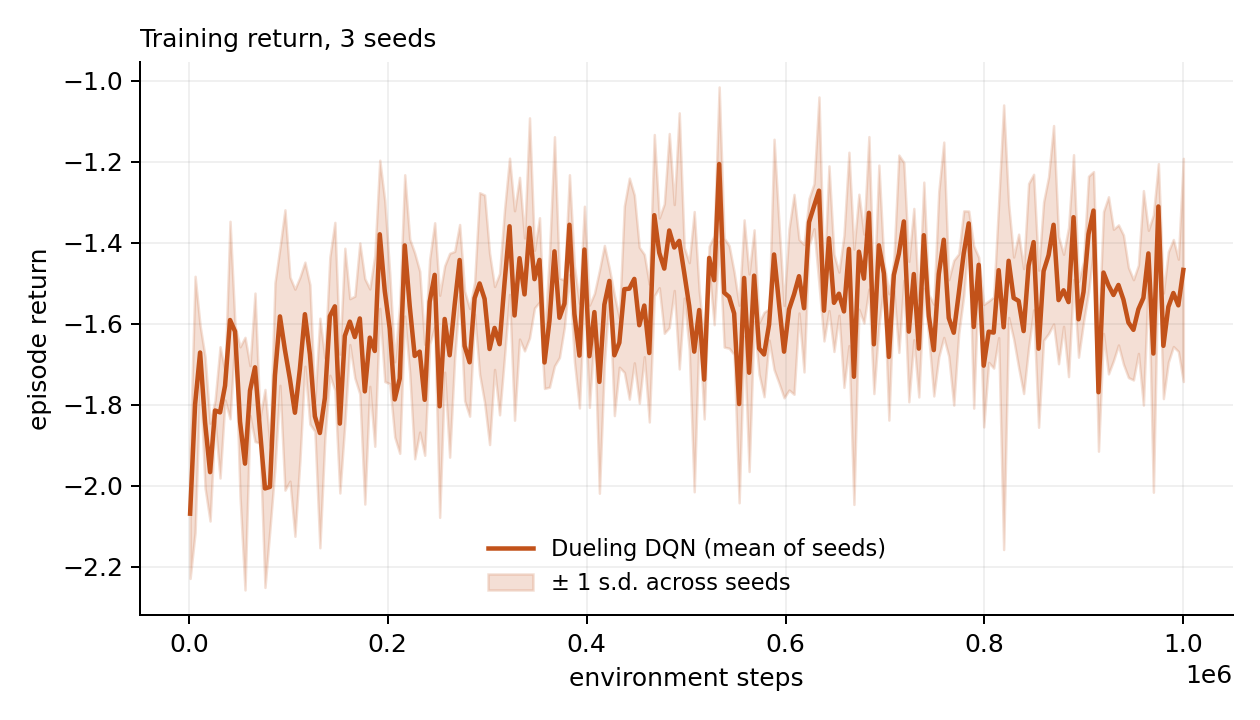
\includegraphics[width=0.72\textwidth]{figures/training_curve.png}
\caption{Episode return against environment steps, averaged across three seeds with a band at one
standard deviation.}
\label{fig:training}
\end{figure*}

\subsection{Training}\label{training}

Figure~\ref{fig:training} plots episode return against environment steps, averaged across seeds.
Return rises from -1.79 at 100,000 steps to -1.52 at 400,000 and is flat thereafter, so the budget
sufficed, and the seed spread stays at or below 0.041. Training returns include $\epsilon$ = 0.05 and are
not comparable to evaluation numbers.

\subsection{Dispatching rules}\label{the-dispatching-rules-and-the-bar-they-set}

{\def\LTcaptype{none} % do not increment counter
\begin{table*}[t]
\centering\small
\caption{The eight dispatching rules on the thirty held-out instances.}
\label{tab:rules}
\begin{tabular}{lrrrr}
\toprule
Rule & Avg.\ waiting & Missed & Weighted tardiness & Return \\
\midrule
SPT ($=$ SJF) & 4.077 & 0.256 & 136.4 & $-1.352$ \\
WSPT & 4.344 & 0.276 & 104.9 & $-1.187$ \\
ATC  & 4.372 & 0.277 & 95.1  & $-1.125$ \\
EDD  & 4.521 & 0.363 & 124.0 & $-1.345$ \\
CR   & 4.851 & 0.445 & 133.8 & $-1.465$ \\
MS   & 4.947 & 0.421 & 144.8 & $-1.554$ \\
FCFS & 5.539 & 0.465 & 212.3 & $-2.099$ \\
LPT  & 7.744 & 0.421 & 437.9 & $-3.958$ \\
\bottomrule
\end{tabular}
\end{table*}

}

Table~\ref{tab:rules} lists the eight rules on the held-out instances, ordered by return; two
rules inside the action set beat all three required baselines. ATC at -1.125 is the reference,
since a Formulation B policy that always selects it reaches that score.


\begin{figure*}[t]
\centering
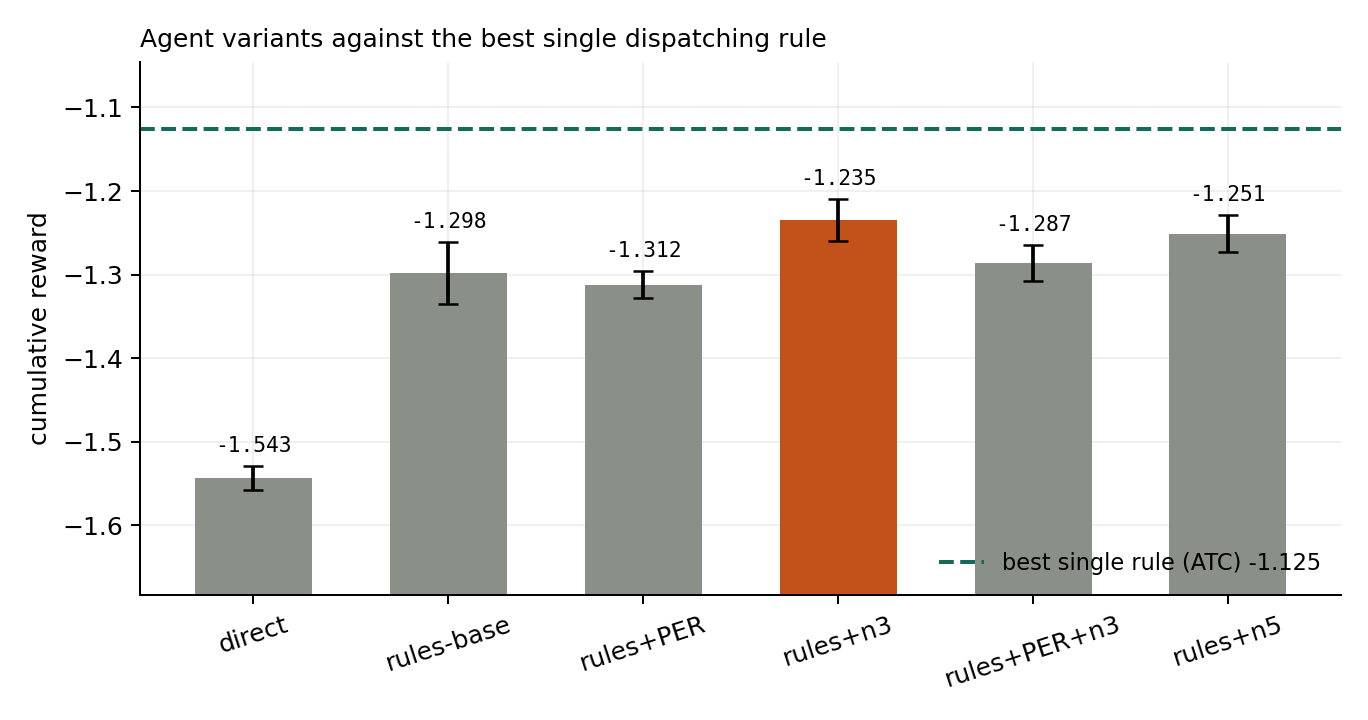
\includegraphics[width=0.72\textwidth]{figures/ablation.png}
\caption{Agent variants against the best single dispatching rule. The dashed line is ATC at
$-1.125$. Every variant on the rule action space outperforms all three required baselines; none reaches
ATC.}
\label{fig:ablation}
\end{figure*}

\subsection{Ablation}\label{ablation}

{\def\LTcaptype{none} % do not increment counter
\begin{table*}[t]
\centering\small
\caption{Ablation across three seeds at one million steps per seed.}
\label{tab:ablation}
\begin{tabular}{lcccc}
\toprule
Variant & Per-seed return & Mean & s.d. & Gap to ATC \\
\midrule
Formulation A, direct assignment & $-1.525$, $-1.544$, $-1.561$ & $-1.543$ & 0.015 & $-0.418$ \\
Formulation B, uniform replay    & $-1.334$, $-1.314$, $-1.247$ & $-1.298$ & 0.037 & $-0.173$ \\
B $+$ prioritised replay         & $-1.309$, $-1.333$, $-1.294$ & $-1.312$ & 0.016 & $-0.187$ \\
B $+$ n-step 3                   & $-1.222$, $-1.212$, $-1.269$ & $-1.235$ & 0.025 & $-0.109$ \\
B $+$ PER $+$ n-step 3           & $-1.315$, $-1.282$, $-1.263$ & $-1.287$ & 0.021 & $-0.161$ \\
\bottomrule
\end{tabular}
\end{table*}

}

Table~\ref{tab:ablation} gives per-seed and mean return for each variant, and
Figure~\ref{fig:ablation} plots the means against ATC. We compare differences against the
combined seed spread, with per-seed dominance checked.

\begin{itemize}
\item
  The action space is the largest of the three effects tested. Formulation B improves on A by
  0.245, far beyond any spread, and every B variant outperforms all three required baselines,
  whereas A outperforms only First-Come-First-Served.
\item
  n-step returns help: +0.064 against a combined spread of 0.062, winning on every seed.
\item
  Prioritised replay does not: -0.014 against a spread of 0.053, no per-seed dominance, and a 0.052
  degradation on top of n-step.
\end{itemize}

\subsection{Headline result}\label{headline-result}

The best configuration is Formulation B with n-step 3 returns, at -1.235 $\pm$ 0.025. It beats
First-Come-First-Served and Round Robin on every metric and every seed, and Shortest-Job-First on
return, weighted tardiness (107.6 against 136.4) and makespan. Shortest-Job-First retains the lower
average waiting time (4.077 against 4.525) and fewer missed deadlines (0.256 against 0.354). In
return the agent improves on First-Come-First-Served by 0.864, on Shortest-Job-First by 0.117 and
on Round Robin by 0.164, all beyond the seed spread.

ATC scores -1.125 against the agent's -1.235, a difference of 0.109 that exceeds the seed
spread; §6.4 discusses the cause.

Figure~\ref{fig:bars} shows every policy on the four metrics. Machine utilisation (0.884--0.927)
and makespan vary by under 5\% across all thirteen policies; both are dominated by the arrival process, and are reported for completeness.


\begin{figure*}[t]
\centering
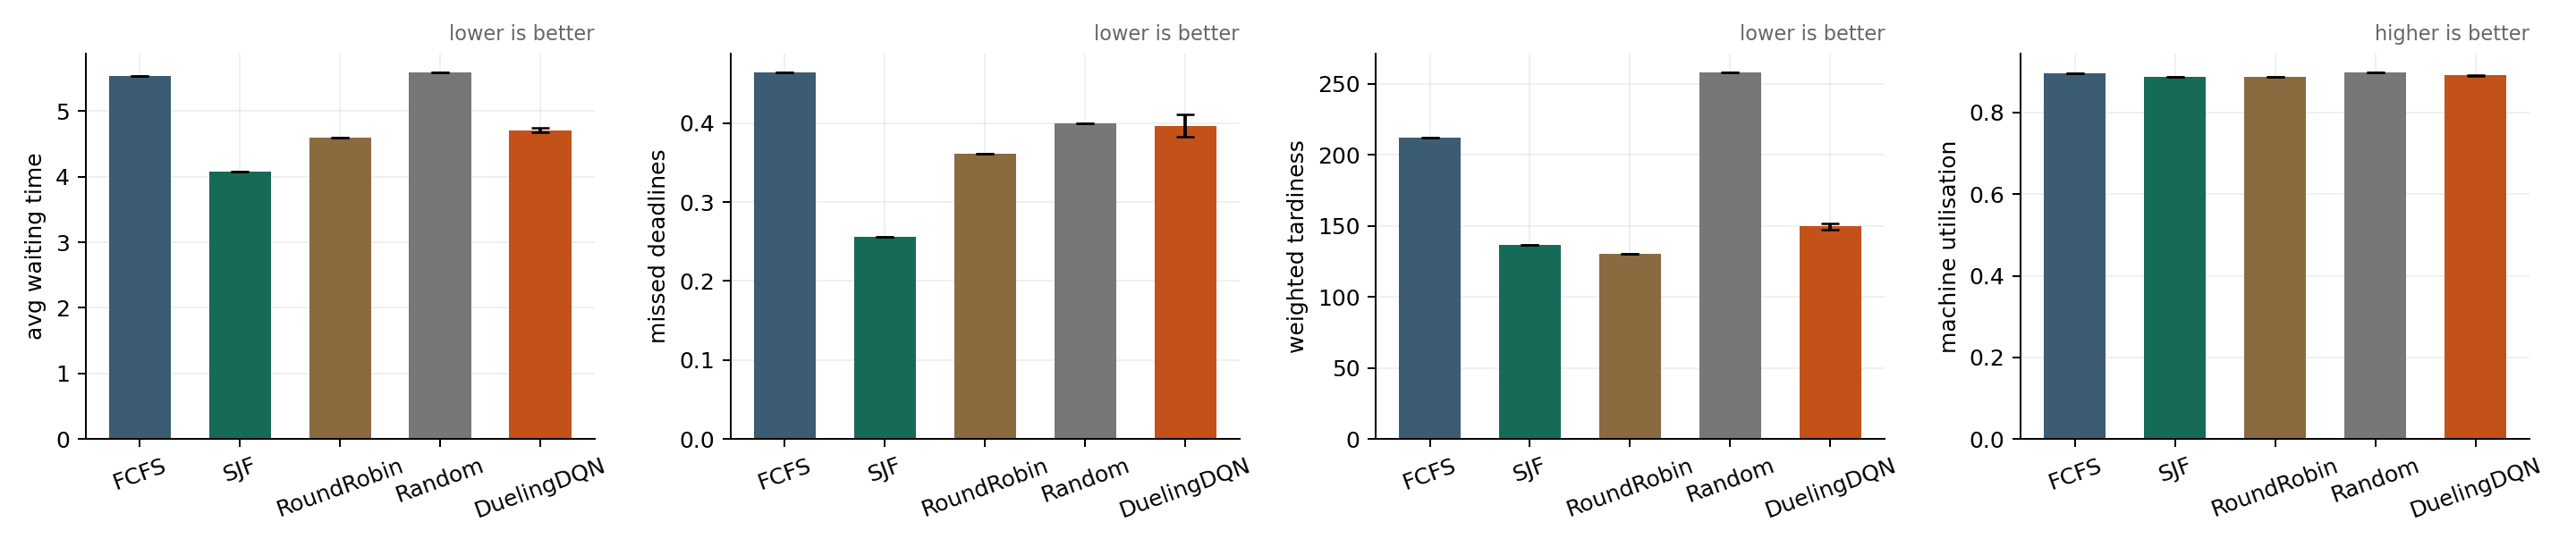
\includegraphics[width=\textwidth]{figures/baseline_bars.png}
\caption{Every policy on four metrics, error bars from the spread across seeds. Utilisation and
makespan barely separate the policies at this load.}
\label{fig:bars}
\end{figure*}

\section{Discussion}\label{discussion}

\subsection{Action space}\label{the-action-space-was-the-binding-constraint}

Formulation B improves on A by 0.245 in return, an order of magnitude larger than any other change
tested. Under A the agent outperformed only First-Come-First-Served, whereas under B every variant
outperforms all three required baselines.

The mechanism lies in the state encoding: SPT implements a comparison across queued jobs, which
under A the network must learn from a flat 69-dimensional vector in which each slot occupies a
fixed, arbitrary offset. Under B the rule performs the comparison and the network need only represent \emph{when}
each rule applies. The measured Q-spread of 0.11 across legal actions, against episode
returns near -2, supports this: state value was estimated well and between-action ordering poorly.

\subsection{Prioritised replay}\label{prioritised-replay-did-not-help-contrary-to-our-own-prediction}

Our literature review recommended prioritised replay as the highest-value change, because it is
part of the recipe of the closest precedent. The ablation does not support this: -0.014 against
a combined spread of 0.053, with no per-seed dominance.

This result does not refute \citet{hanyang2020}. Their CNN-over-images state, their 85 static
OR-Library instances and their dueling double DQN all differ from our setting, and any of those
could change the value of prioritising by temporal-difference error. Our review found no
scheduling-domain ablation isolating prioritised replay.

The mechanism fits the diagnosis in §6.1. Reward is 0 when a dispatch is committed and its cost
appears tens of decisions later, and n-step propagates that consequence to the causing action.
Prioritised replay changes which transitions are replayed, not how far credit is propagated.

\subsection{Development faults}\label{three-faults-found-by-measuring-rather-than-assuming}

The action space originally included a no-op, and the no-op was selected at 46.3\% of decision
epochs, scoring
worse than a uniform-random legal policy. Training instance seeds for two of three seeds fell
inside the held-out evaluation range, which would have inflated the headline numbers. The loss
supplied an all-ones current-state mask, so \texttt{Q(s,a)} during the update differed from what the
behaviour policy evaluated, and performance degraded with training. None of the three raised an
error; each was found by a diagnostic check run before the result was accepted, and Appendix A
gives the forensics and the tests.

\subsection{ATC gap}\label{why-the-agent-stops-short-of-the-best-single-rule}

Return plateaus from 400,000 steps with a seed spread under 0.05, so more compute does not close
the gap, and the reward ranking and the metric ranking agree, with ATC top of both, so a better score on this reward is a better schedule.

The remaining constraint is the state representation: under Formulation B the network selects a
rule for the current queue from a flat concatenation of ten slots.
Prior work addresses this with a structured encoder, either a graph network over the disjunctive
representation or attention over the queue, which makes cross-job comparison native. That is the
leading item in further work.

\subsection{Exploration}\label{exploration}

Exploration is $\epsilon$-greedy and uniform over the legal actions, with $\epsilon$ decaying from 1.0 to 0.05 over
the first 30\% of training and held there. Sampling from the legal set rather than all 51 outputs
matters at this action size. Under a typical mask most of the full space is illegal, and uniform
sampling would spend the budget on actions the environment rejects. We conducted no hyperparameter
search, so the schedule is the standard DQN default. The evidence that it sufficed is the return curve in
§5.1, flat over the last 600,000 steps at $\epsilon$ = 0.05.

\section{Limitations and deployment}\label{limitations-and-deployment-considerations}

The state is only partially observed: just the ten most urgent queued jobs are visible, and the
arrival times of unreleased jobs are absent. A recurrent encoder, or stacking a short observation
history, is the natural response and we did not attempt it.

Masking the no-op removes a capability an operator would want, namely holding a fast machine for an
urgent job arriving imminently. The cause is a reward whose per-step signal is almost always
negative, which makes deferral attractive under discounting. Potential-based shaping would likely
let the no-op be retained, but testing that was out of scope.

The instance distribution is synthetic and single-operation, whereas real job shops have
multi-operation jobs with precedence constraints, sequence-dependent setups, breakdowns and
non-stationary arrivals. Transfer to those settings was not tested, and the load parameters were
chosen partly to make the comparison informative. Three seeds is a small sample, so differences are compared
against the seed spread and no significance test is supported.

For deployment, inference is one forward pass through a small network, fast enough for a dispatch loop. The mask is enforced by the
environment, so an out-of-distribution observation cannot produce an illegal schedule, and the
failure mode is a poor legal choice rather than an invalid one. Under Formulation B every action is
a named dispatching rule, so an operator can audit each decision. However, the policy is specific to its training arrival
distribution, so a shift in load requires retraining.

\section{Conclusion and further work}\label{conclusion-and-further-work}

We formulated dynamic job scheduling on heterogeneous parallel machines as a masked-action MDP and
trained a Dueling DQN on it under two action formulations. The comparison ran on held-out instances
under a protocol fixed in advance, against three required dispatching rules and the best of eight.
The rule formulation with three-step returns beats all three required baselines in return on
every seed, and scores 0.109 below the strongest rule in its own action set.

Three problems found during development raised no error: an instance-seed overlap with the
held-out set, a mask omitted from the loss, and a reward structure that rewarded stalling. Each was
found by a diagnostic check, a uniform-random legal policy or a load-separation test.

Further work, in order of expected value: replace the fixed ten-slot window with a
permutation-invariant encoder over the queue; retain the no-op under potential-based shaping;
evaluate \texttt{double\_q} as the D3QN combination standard in the literature; and test transfer across
untrained arrival rates.

\begin{center}\rule{0.5\linewidth}{0.5pt}\end{center}
